\documentclass[a4paper]{report}

%====================== PACKAGES ======================

\usepackage[french]{babel}
\usepackage[utf8x]{inputenc}
%pour gérer les positionnement d'images
\usepackage{float}
\usepackage{amsmath}
\usepackage{graphicx}
\usepackage[colorinlistoftodos]{todonotes}
\usepackage{url}
%pour les informations sur un document compilé en PDF et les liens externes / internes
\usepackage[colorlinks=true,urlcolor=blue]{hyperref}
%pour la mise en page des tableaux
\usepackage{array}
\usepackage{tabularx}
%pour utiliser \floatbarrier
%\usepackage{placeins}
%\usepackage{floatrow}
%espacement entre les lignes
\usepackage{setspace}
%modifier la mise en page de l'abstract
\usepackage{abstract}
%police et mise en page (marges) du document
\usepackage[T1]{fontenc}
\usepackage[top=2cm, bottom=2cm, left=2cm, right=2cm]{geometry}
%Pour les galerie d'images
\usepackage{subfig}
%multirow table
\usepackage{multirow}
%Source code
\usepackage{listings}

\usepackage{color}
\usepackage{hhline}

\definecolor{pblue}{rgb}{0.13,0.13,1}
\definecolor{pgreen}{rgb}{0,0.5,0}
\definecolor{pred}{rgb}{0.9,0,0}
\definecolor{pgrey}{rgb}{0.46,0.45,0.48}

\usepackage{listings}
\usepackage{url}
\lstdefinestyle{numbers} {numbers=left, stepnumer=1, numberstyle=\tiny, numbersep=10pt}
\lstdefinestyle{MyFrame}{backgroundcolor=\color{white},frame=shadowbox}

\lstdefinestyle{MyBashStyle}{language=bash,style=numbers,style=MyFrame,frames=lines}
\lstdefinestyle{MyPythonStyle}{language=python,style=numbers,style=MyFrame,frame=lines}

\lstset{language=bash,frame=lines}
\lstset{language=python,frame=lines}


%====================== INFORMATION ET REGLES ======================
%rajouter les numérotation pour les \paragraphe et \subparagraphe
\setcounter{secnumdepth}{4}
\setcounter{tocdepth}{4}
\hypersetup{							% Information sur le document
pdfauthor = {Florian GRANTE},			% Auteurs
pdftitle = {Monitoring : Mise en place d'une solution IoT avec Microsoft Azure},			% Titre du document
pdfsubject = {Livrable 1},		% Sujet
pdfkeywords = {IoT, Microsoft, informatique, Azure, Raspberry pi},	% Mots-clefs
pdfstartview={FitH}}					% ajuste la page à la largueur de l'écran
%======================== DEBUT DU DOCUMENT ========================
\begin{document}
%régler l'espacement entre les lignes
\newcommand{\HRule}{\rule{\linewidth}{0.5mm}}
%page de garde
\begin{titlepage}
\begin{center}

% Upper part of the page. The '~' is needed because only works if a paragraph has started.

\includegraphics[width=0.8\textwidth]{./images/logo}~\\[1cm]

\textsc{\LARGE Monitoring : Mise en place d'une solution IoT avec Azure}\\[1.5cm]

\textsc{\Large }\\[0.5cm]

% Title
\HRule \\[0.4cm]

{\huge \bfseries Dossier d'installation\\[0.4cm] }

\HRule \\[1.5cm]

% Author and supervisor
\begin{minipage}{0.4\textwidth}
\begin{flushleft} \large
\emph{Auteur:}\\
Florian \textsc{GRANTE}\\
\end{flushleft}
\end{minipage}
\begin{minipage}{0.4\textwidth}
\begin{flushright} \large
\emph{Superviseur:} \\
David \textsc{LAROSE}
\end{flushright}
\end{minipage}

\vfill

% Bottom of the page
{\large \today}

\end{center}
\end{titlepage}
%ne pas numéroter cette page
\thispagestyle{empty}
%\newpage
%%%\input{./abstract.tex}
\tableofcontents
\thispagestyle{empty}
\setcounter{page}{0}
%ne pas numéroter le sommaire
%\newpage
%espacement entre les lignes d'un tableau
\renewcommand{\arraystretch}{1.5}
%====================== INCLUSION DES PARTIES ======================
~
\thispagestyle{empty}
%recommencer la numérotation des pages à "1"
\setcounter{page}{0}
\newpage
\chapter*{Introduction}

\addcontentsline{toc}{chapter}{Introduction}


L'objectif de ce dossier est de vous expliquer de A à Z la mise en place d'un système avec capteurs permettant l'affichage en temps réel de différentes données comme la température, l'humidité ou encore la luminosité d'une pièce, d'un couloir, etc....

En premier lieu, nous allons nous attarder sur la partie matériel : \textit{La Raspberry Pi} (je vous laisserais le choix du genre, c'est une question qui divise la France comme bien d'autre)

\begin{figure}[H]
\begin{center}
	\makebox[\textwidth]{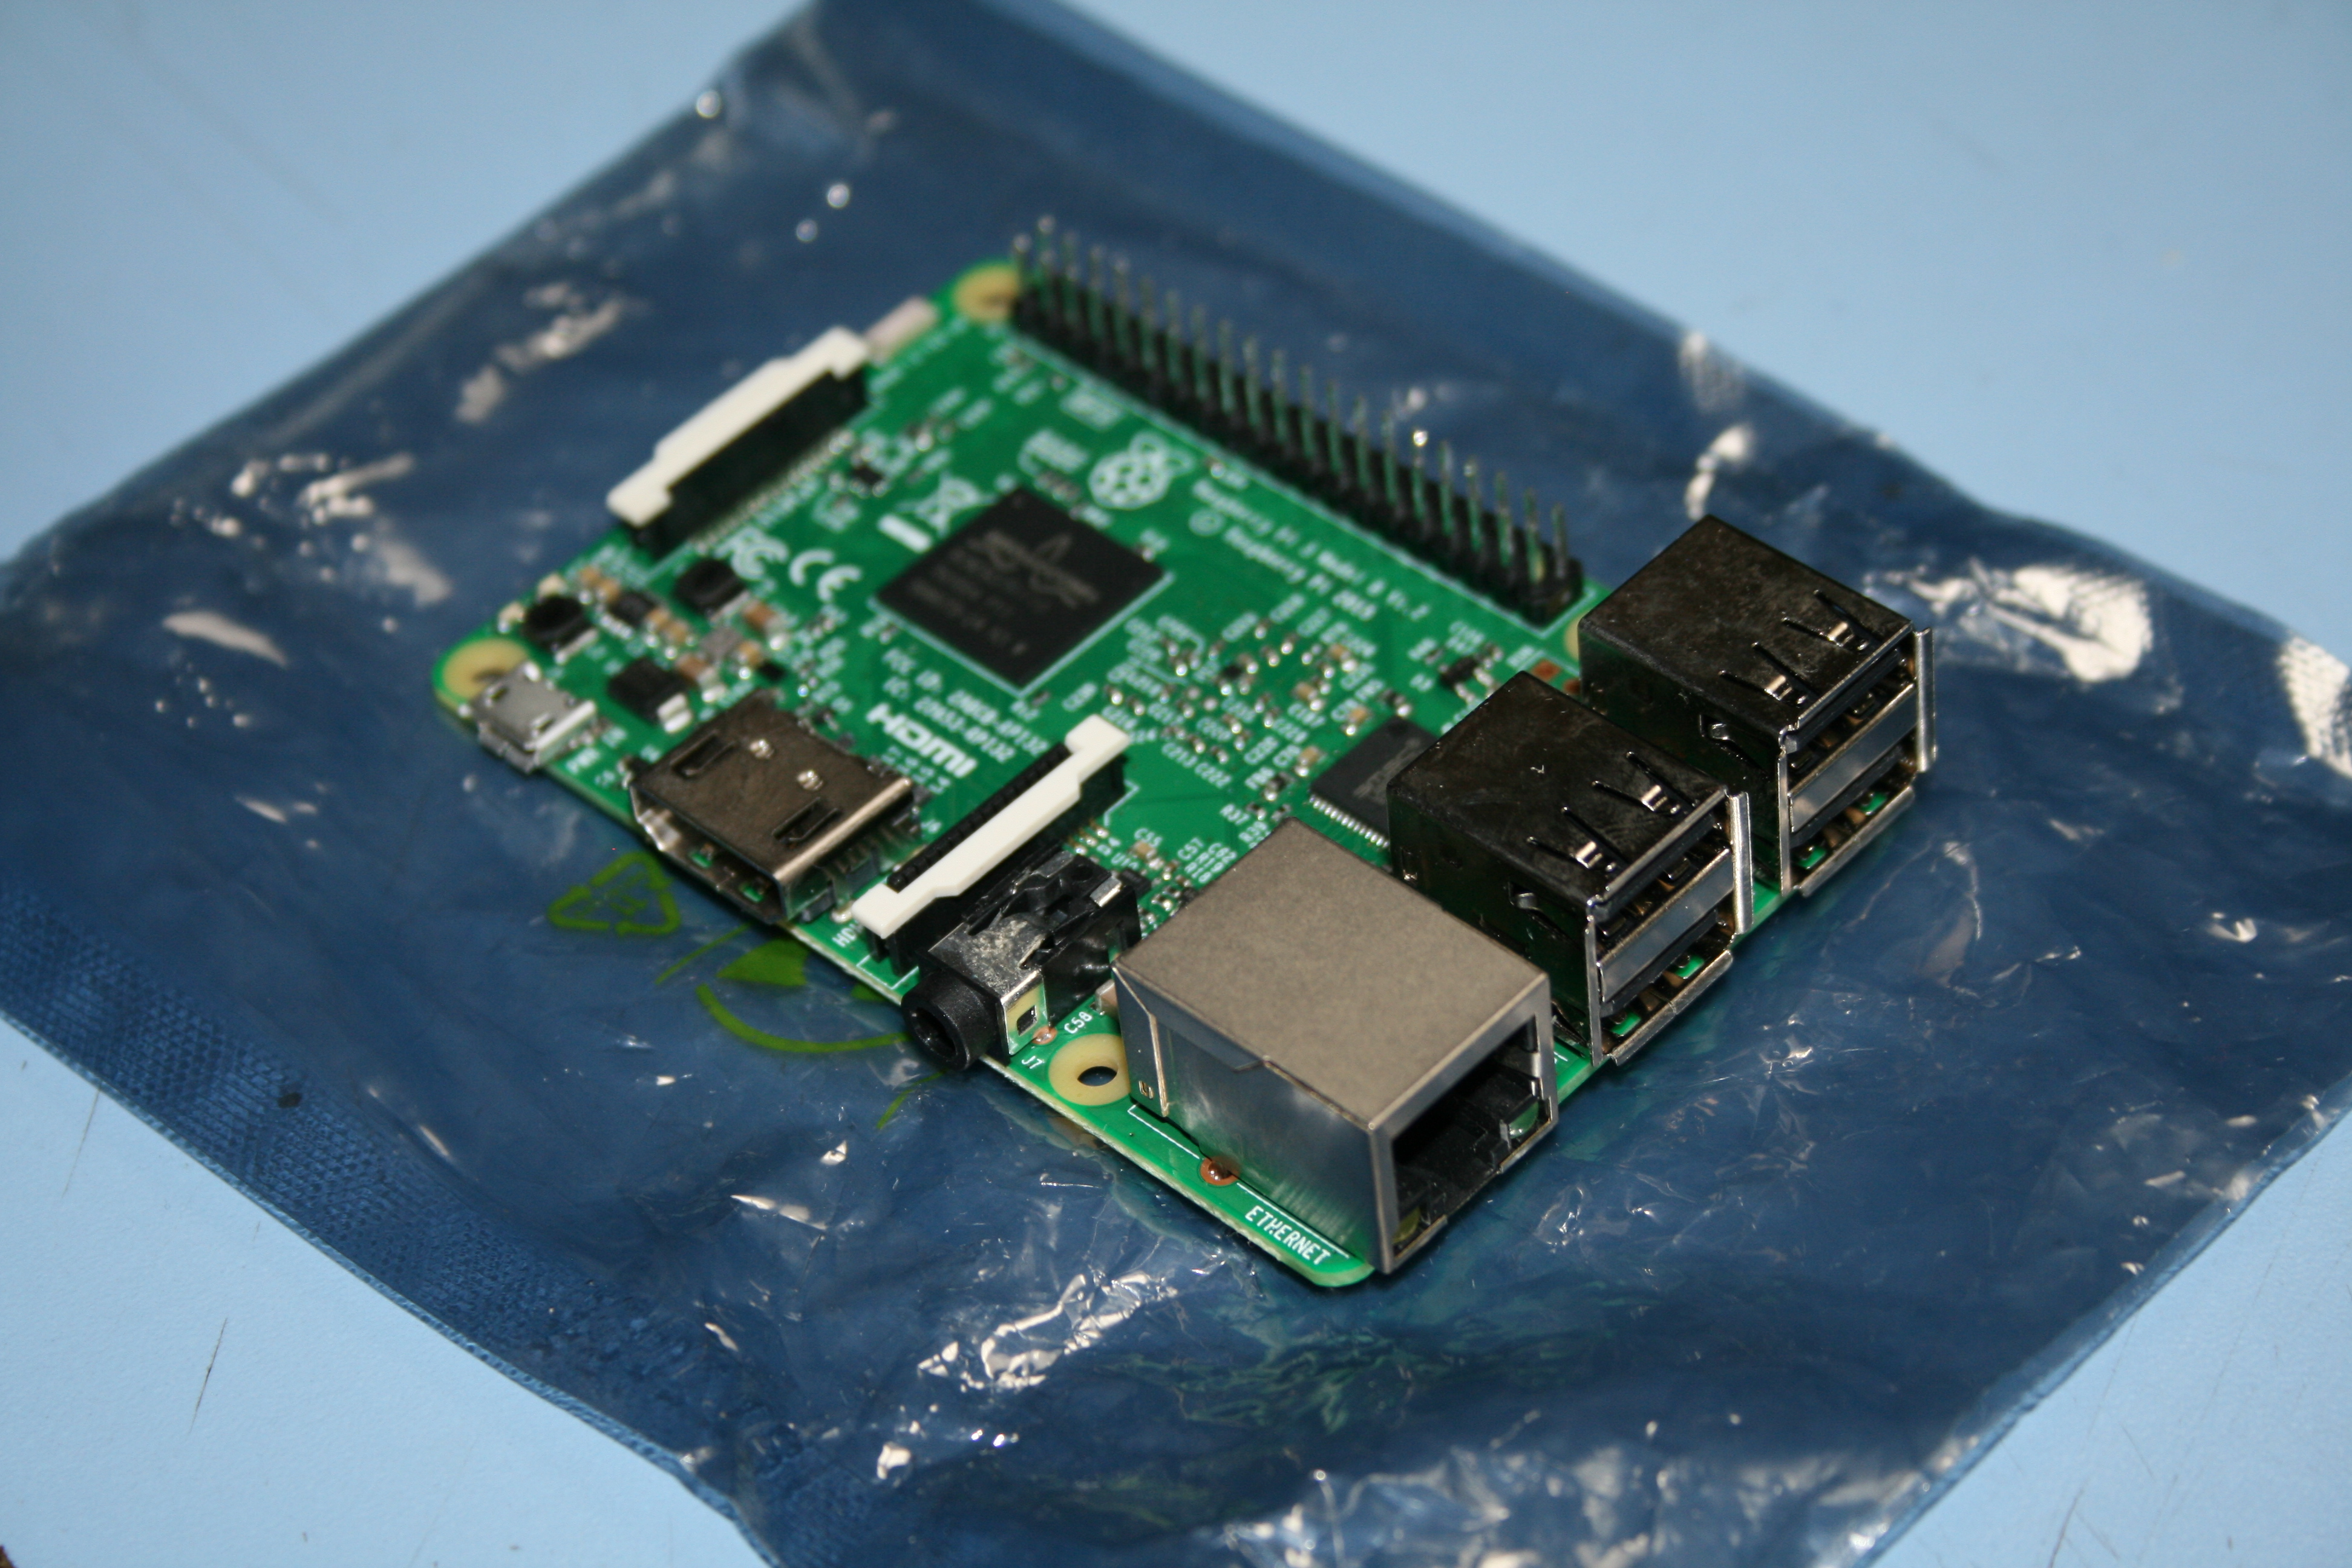
\includegraphics[width=.7\paperwidth]{images/rpi.jpg}}
\end{center}
	\caption{ \textit{Une RaspberryPi à nue}}
\end{figure}

Nous aborderons l'installation de capteur sur cette carte puis nous verrons l'installation logiciel.

Dans un second temps, nous verrons ensemble comment envoyer ces données dans le \textit{Cloud} mis en place par \textit{Microsoft} : \textit{Azure} 

A la fin de ce dossier, vous serez en mesure de regarder n'importe où dans le monde la température ambiante de votre installation mais cessons de tergiverser et mettons nous au travail !
\chapter{Présentation du matériel}

\section{La \textit{RaspberryPi}}

Si vous avez été intriguer par la bête que je vous ai mis en photo dans l'introduction, pas de panique, elle va devenir votre nouvelle meilleure amie. Il s'agit ni plus ni moins que d'un ordinateur en modèle réduit.
Cette puce est capable de faire tourner une distribution de \textit{Linux} connue sous le nom de \textit{Raspbian}. La \textit{RaspberryPi} est un véritable bijoux de miniaturisation pour les \textit{Makers} qui désire embarquer des ordinateurs dans leur projets les plus fou. Vous l'aurez compris, cela va être notre base de notre station.\\

\textit{Pourquoi ce choix ? }\\

La \textit{RaspberryPi} peut être repoussante au début car vendue tel que vous avez pu la voir  plus tôt mais une fois prise en main, elle est simple d'utilisation. Elle permet d'avoir un accès internet de façon simple avec son port ethernet, on peut y brancher un écran ainsi que des périphériques si nécessaire pour réaliser de la maintenance (même si il existe d'autre moyen d'y accéder mais nous verrons ça plus tard). 
Une raison non négligeable pour notre projet est son prix. Compté une quarantaine d'euros pour le dernier modèle en date.
Elle possède également des broches pour réaliser de l'électronique embarquée comme nous allons le faire. Ainsi notre ordinateur est modulaire et on peut y ajouter des composants par ces broches.\\

\begin{figure}[H]
\begin{center}
	\makebox[\textwidth]{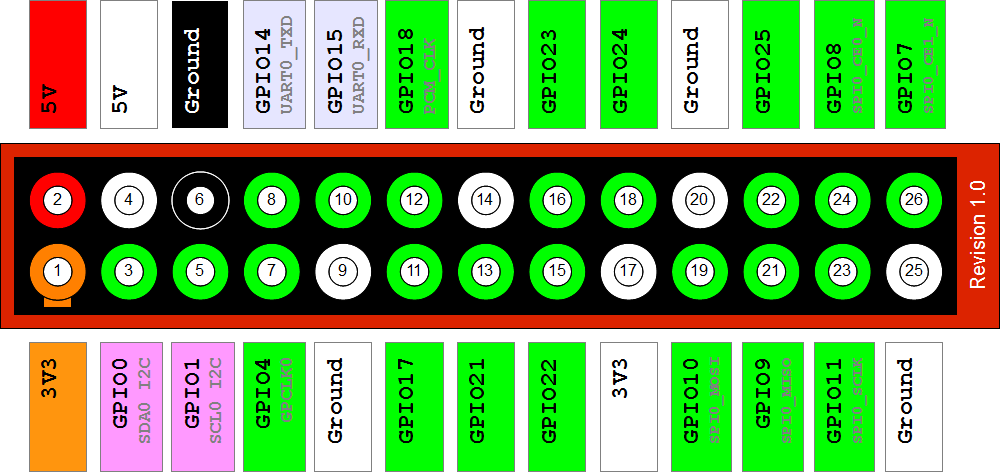
\includegraphics[width=.7\paperwidth]{images/pinrpi.png}}
\end{center}
	\caption{ \textit{Pin Mapping de la RaspberryPi 3}}
\end{figure}\\

Son autre atout et non des moindre, c'est sa communauté qui s'est étendue de façon exponentielle ces dernières années car accessible à tout le monde et permet alors une aide conséquente via les forums.

Vous voilà plus familier avec l'engin, si vous voulez plus d'information, je vous laisse visiter \href{https://www.raspberrypi.org/}{le site officiel} où vous pouvez notamment télécharger la version de base de son OS, \textit{Raspbian} mais qui possède nombre de version modifié (un OS pour réaliser une station de jeux rétro est un exemple)

\section{Le shield \textit{GrovePi+}}

Je vous parlait juste avant que la \textit{RaspeberryPi} possédait des broches. Ces dernière vont nous servir à y installer les capteurs. Mais nous n'allons pas brancher les capteurs directement sur la \textit{RaspberryPi}. En effet nous allons ajouter ce que l'on appelle un \textit{"Shield}. Il s'agit ni plus ni moins que d'une autre carte électronique avec ses fonctions propre qui se branche sur la \textit{RaspberryPi} pour communiquer avec elle. Ainsi, nous pouvons utiliser les fonctions du \textit{"Shield"} en envoyant des instruction de puis la \textit{"RaspberryPi}.

Celui que nous utilisons porte le doux nom \textit{GrovePi+}. Sans m'attardez sur ses détails techniques, sachez (pour les connaisseurs) qu'elle embarque un microcontrôleur ATMega pour gérer les capteurs. Il s'agit ni plus ni moins d'une version \textit{"User Friendly"} d'un \textit{Arduino} que l'on branche sur notre \textit{RaspberryPi}.\\

\begin{figure}[H]
\begin{center}
	\makebox[\textwidth]{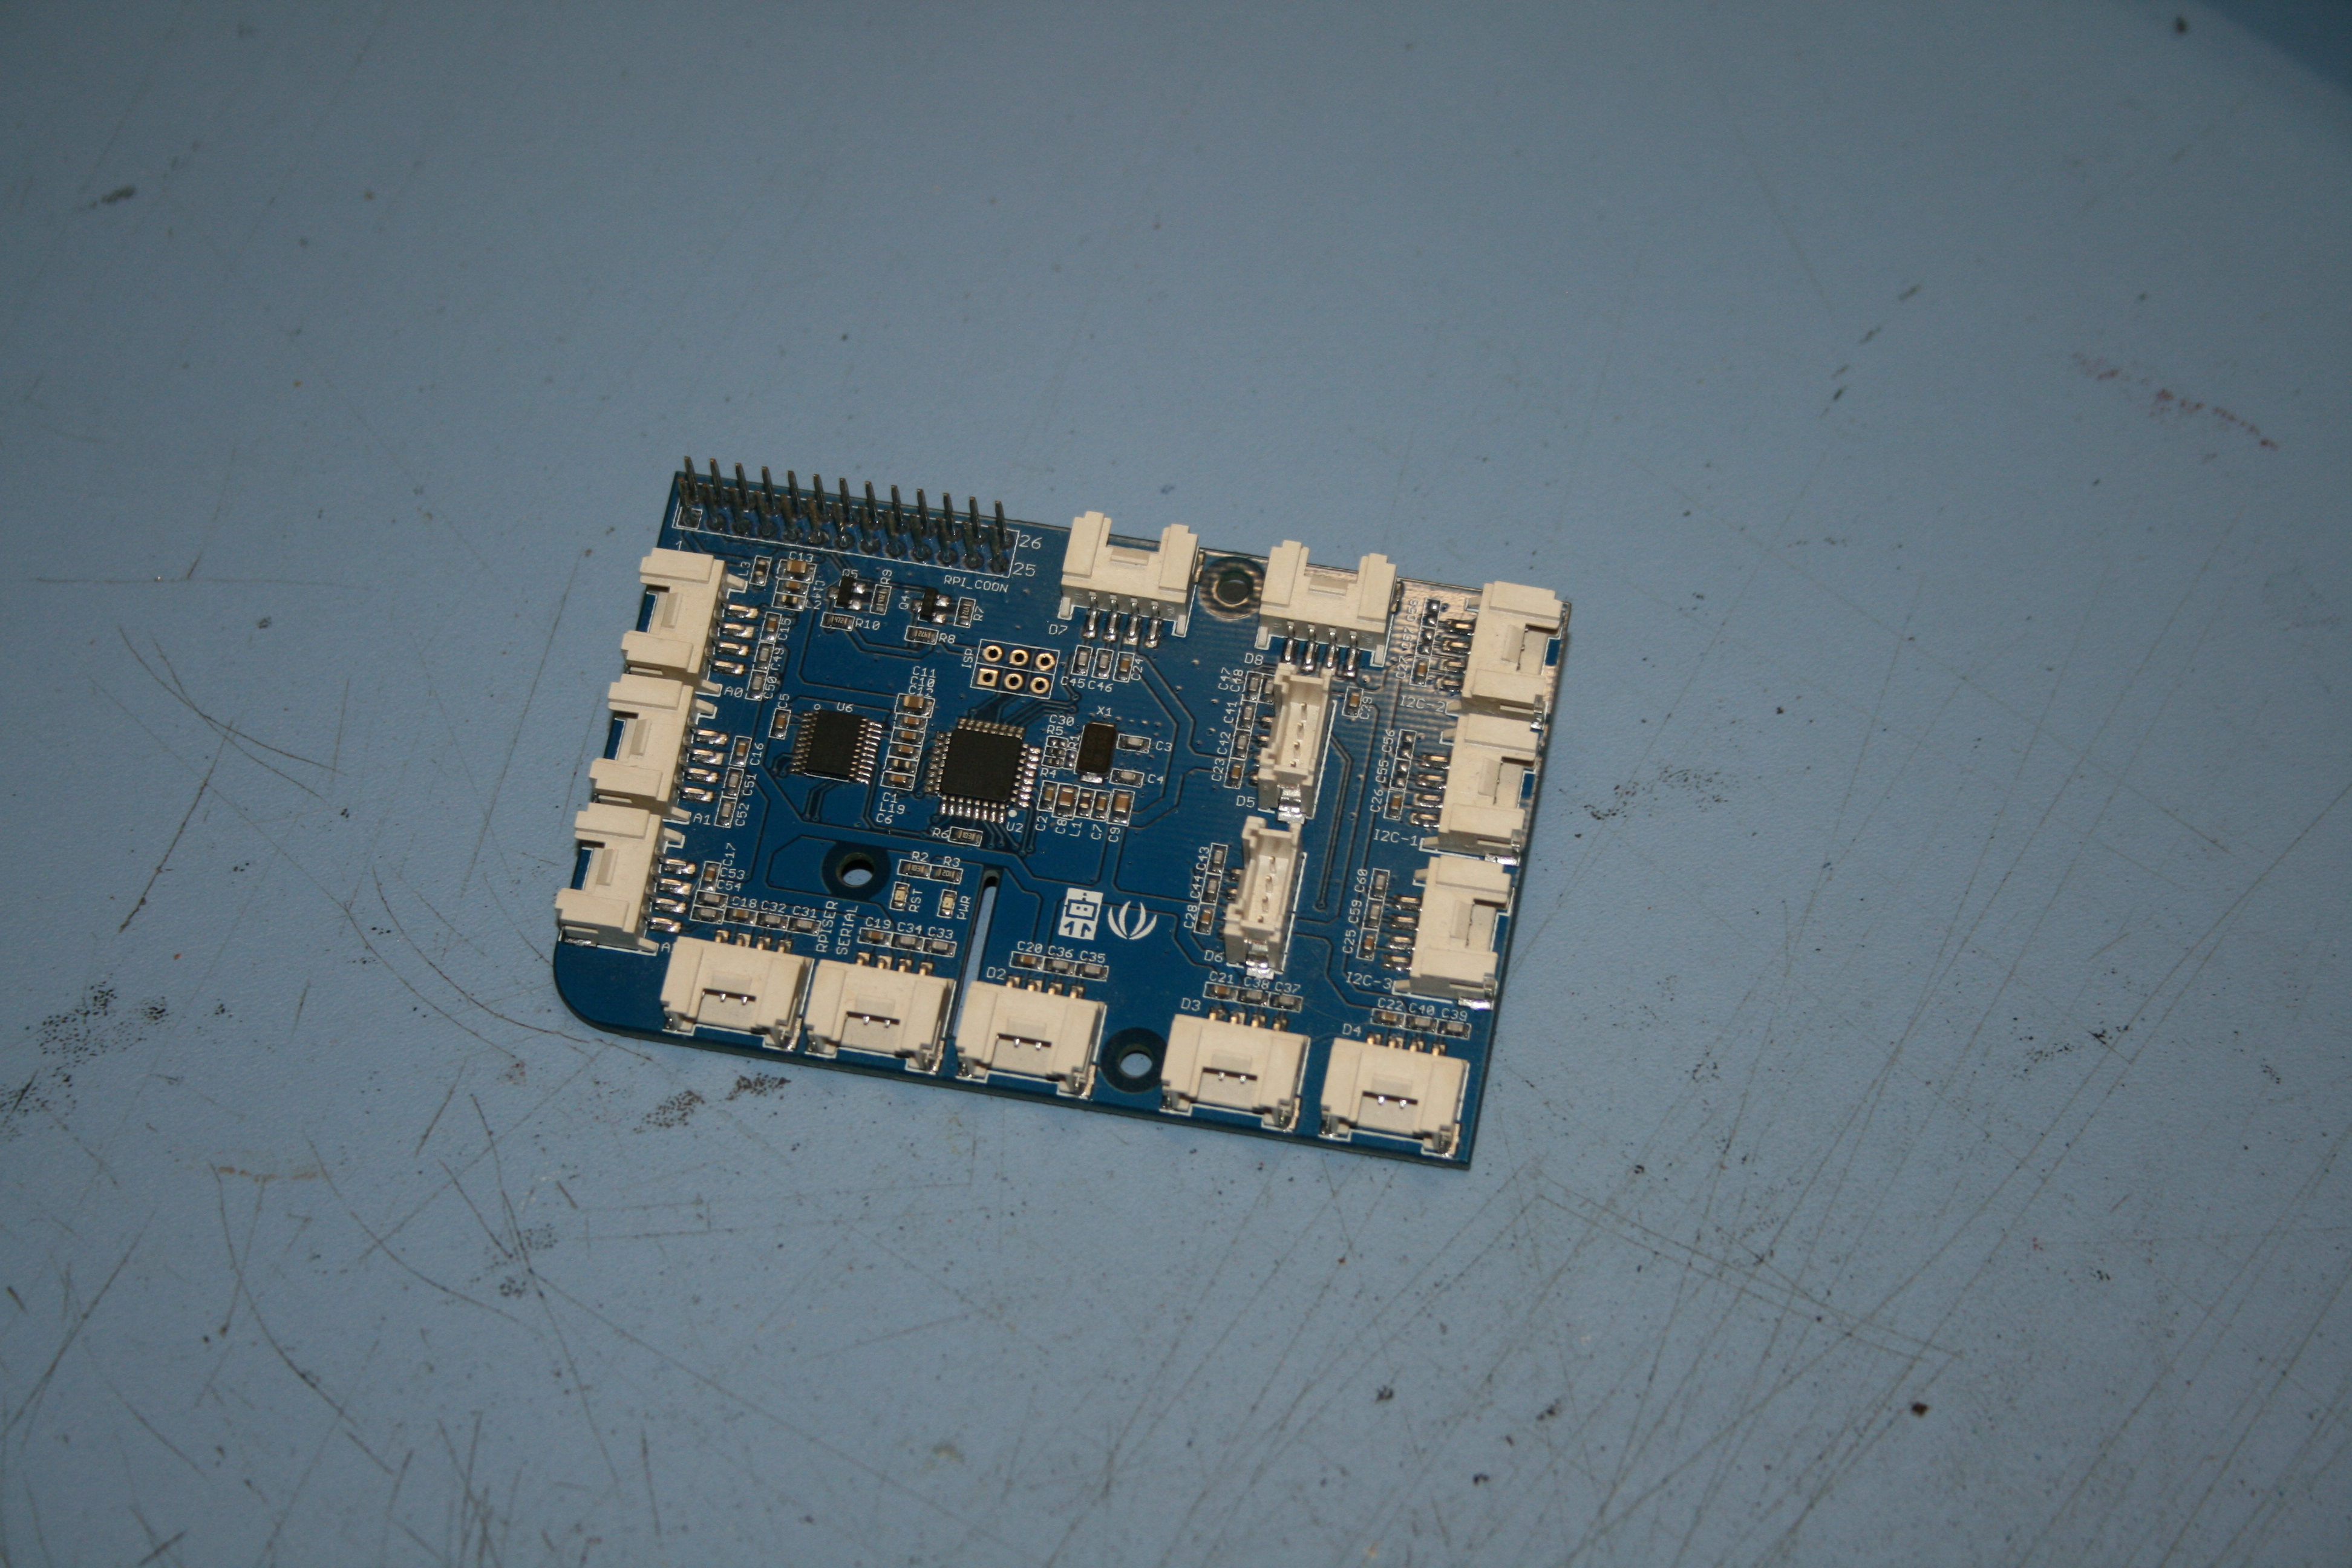
\includegraphics[width=.7\paperwidth]{images/grovepi.jpg}}
\end{center}
	\caption{ \textit{le Shield GrovePi+}}
\end{figure}\\


Comme vous voyer sur la photo, nous avons des connecteurs \textit{4-pins}, en blanc. C'est là dessus que l'on va brancher nos capteurs.\\
\\
\textbf{ATTENTION : Ces connecteurs sont reliés à des broches particulière du microcontrôleur. Ils sont donc chacun d'entre eux prévu pour un type de composant particulier. } \\

On distingue trois types de connecteurs parmis ceux-là :

\begin{itemize}
	\item ports analogiques : Ils sont disponible uniquement en \textit{INPUT}, c'est à dire qu'il s'agit d'une entrée pour une tension comprise entre 0 et 5V. Le \textit{Shield} possède un convertisseur analogique numérique qui échantillonne cette valeur sur 10bits (0V = 0 et 5V = 1023. Exemple si on envoie 2.5V, alors on aura la valeur 512)
	
	\item ports digitaux : ceux ci peuvent être régler en \textit{INPUT} ou en \textit{OUTPUT}. Comme ce sont des entrée/sortie numérique, elle répond à la loi du tout ou rien. Soit nous avons 0V, soit nous avons 5V (0 ou 1). Typiquement, pour une sortie cela peut être utilisé comme interrupteur électronique.
	\item ports I2C : Il s'agit d'un protocole de communication développé par Philips pour minimiser le nombre de fil nécessaire pour faire communiquer deux périphériques entre eux. Il y a en effet uniquement 3 fils : un signal de données (SDA), un signal d'horloge (SCL), et un signal de référence électrique (masse).
\end{itemize}

Nous allons maintenant parler rapidement des différents capteurs et composants que nous allons brancher sur notre \textit{Shield}

\section{Les composants}

\subsection{Le capteur de température et d'humidité}

Les capteurs d'humidité répondent à une loi qui dépend de la température. C'est pour cette raison que ces capteurs fournissent bien souvent les deux à la fois. De notre côté, il s'agit du capteur \textit{DHT11}. Ce composant utilise un connecteur digital\\

\begin{figure}[H]
\begin{center}
	\makebox[\textwidth]{\includegraphics[width=.5\paperwidth]{images/dht11.jpg}}
\end{center}
	\caption{ \textit{Capteur d'humidité et de température}}
\end{figure}\\

\href{https://akizukidenshi.com/download/ds/aosong/DHT11.pdf}{Datasheet du DHT11}

\subsection{Le capteur de luminosité}

Le capteur de luminosité mesure la lumière ambiante. Exprimé en Luxmètre, les capteurs de luminosité "basique" ne permettent pas d'obtenir une valeur précise de la luminosité. Néanmoins, cette valeur est très abstraite pour l'utilisateur. C'est pour cette raison que nous allons l'utiliser pour déterminer si la lumière de la pièce où il est placé est allumé ou non. Nous détaillerons un protocole à réaliser pour essayer de faire marcher au mieux ce capteur. Ce composant utilise un connecteur analogique.\\

\begin{figure}[H]
\begin{center}
	\makebox[\textwidth]{\includegraphics[width=.5\paperwidth]{images/lcd.jpg}}
\end{center}
	\caption{ \textit{L'écran LCD}}
\end{figure}\\

\href{https://github.com/SeeedDocument/Grove_Light_Sensor/raw/master/res/LS06-M%CE%A65_datasheet.pdf}{Datasheet du capteur de luminosité}

\subsection{L'écran}

Pour pouvoir accéder localement aux valeurs des capteurs, nous allons placer un écran.
Nous pouvons afficher 2 lignes de 16 caractère sur ce dernier et choisir la couleur de fond qui est affiché. Ce composant utilise un connecteur I2C.\\

\begin{figure}[H]
\begin{center}
	\makebox[\textwidth]{\includegraphics[width=.5\paperwidth]{images/lcd.jpg}}
\end{center}
	\caption{ \textit{L'écran LCD}}
\end{figure}\\

\subsection{L'encodeur rotatif}

Nous n'allons pas l'utiliser comme un capteur à proprement parler ici mais d'un bouton tournant pour naviguer dans différents affichage sur l'écran. On pourra ainsi passer de l'affichage de la température à l'humidité,etc...\\

\begin{figure}[H]
\begin{center}
	\makebox[\textwidth]{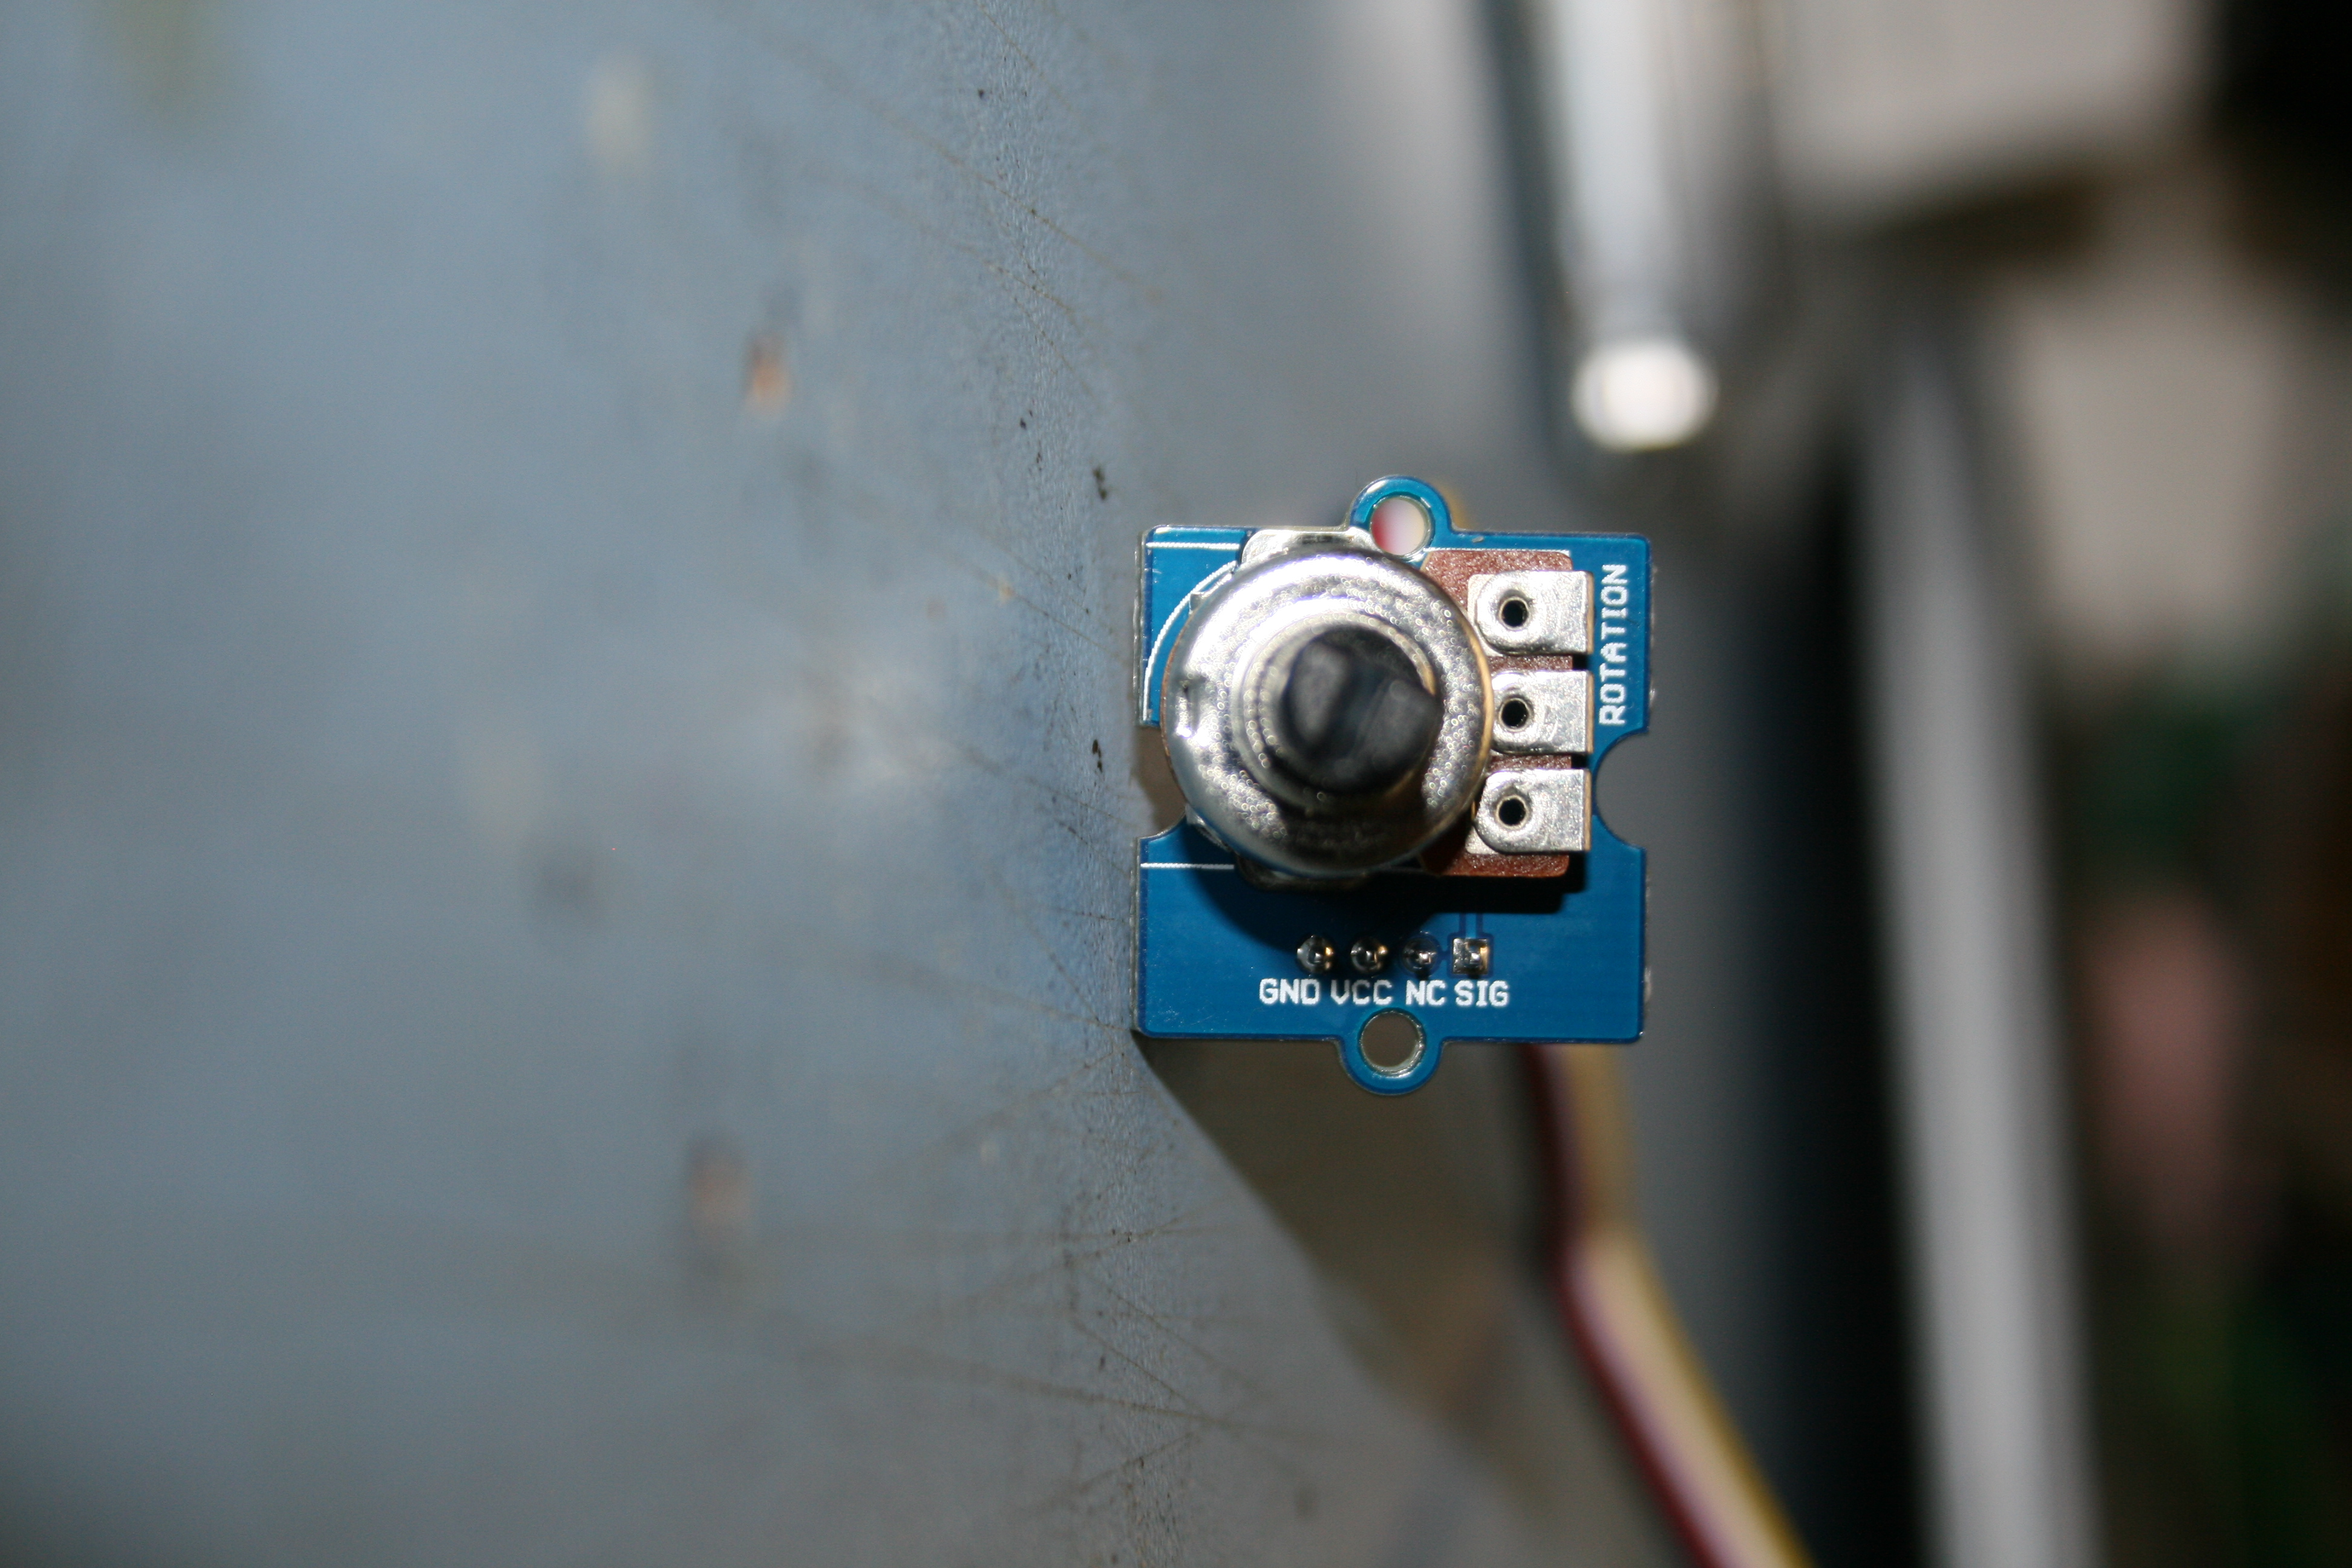
\includegraphics[width=.5\paperwidth]{images/encoder.jpg}}
\end{center}
	\caption{ \textit{Encodeur rotatif pour bouton tournant}}
\end{figure}\\

Maintenant que nous avons connaissance du matériel que nous avons à disposition pour notre station, nous allons pouvoir passer à son installation.






\chapter{Configuration de la station}

\section{Création et installation de la distribution \textit{Raspbian}.}

Pour une \textit{RaspberryPi}, son disque dur est nulle autre qu'une carte Micro SD. C'est donc sur ce support que nous allons faire l'installation.

Pour réaliser cette étape, vous aurez besoin de :
\begin{itemize}
	\item d'une \textit{RaspberryPi}
	\item d'une carte micro SD de minimum 4Go
	\item du logiciel \href{etcher.io}{Etcher}
	\item de \href{https://sourceforge.net/projects/dexterindustriesraspbianflavor/}{\textit{Raspbian}}. En réalité il s'agit d'une version modifiée par la société Dexter Industries qui est spécialisé dans l'utilisation de \textit{RaspberryPi} pour la robotique.
	\item d'un adaptateur pour relier la micro SD à votre ordinateur.
\end{itemize}\\
Nous pouvons désormais commencer l'installation de l'OS sur notre \textit{RaspberryPi}

\begin{enumerate}
	\item Connecter la micro SD sur votre ordinateur.\\
	\item Lancer le logiciel \textit{Etcher}\\
	\begin{figure}[H]
	\begin{center}
		\makebox[\textwidth]{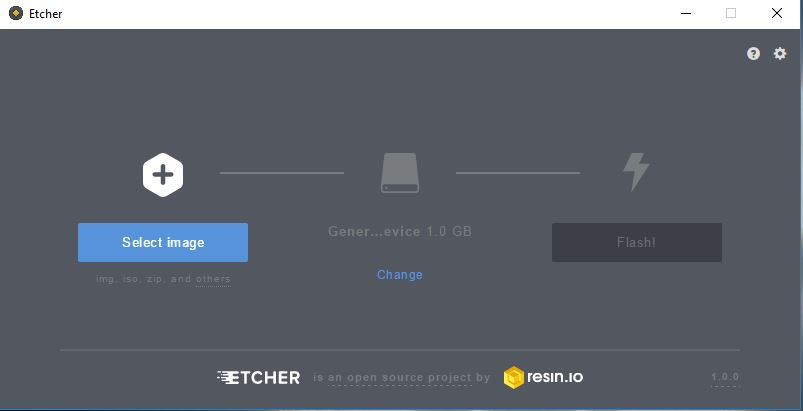
\includegraphics[width=.6\paperwidth]{images/etcher1.jpg}}
	\end{center}
		\caption{ \textit{Logiciel Etcher au lancement}}
	\end{figure}\\
	\item Cliquer sur \textit{"Select image"} à gauche puis sélectionner le fichier \textit{.zip} récupéré depuis le site \textit{SourceForce} dans les pré-requis.\\
	\item Vérifier que le périphérique qui est renseigné au centre est bien la micro SD. Dans le cas contraire cliquer sur \textit{"Change"}.\\
	\item Si les deux étapes précédentes sont OK, cliquer sur \textit{"Flash"}.\\
	\begin{figure}[H]
	\begin{center}
		\makebox[\textwidth]{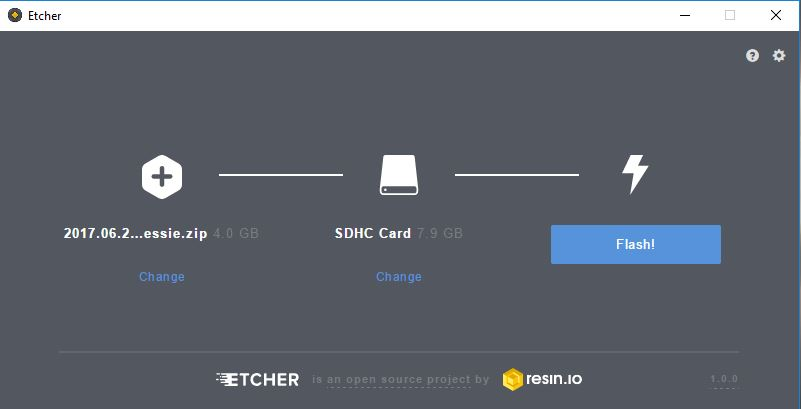
\includegraphics[width=.6\paperwidth]{images/etcher2.jpg}}
	\end{center}
		\caption{ \textit{Etcher prêt à flasher}}
	\end{figure}\\
\end{enumerate}
Et voilà, l'opération peut prendre une dizaine de minutes. C'était simple non ?

\section{Première mise en route de la \textit{RaspberryPi}.}

\begin{enumerate}

	\item Maintenant que vous avez \textit{Raspbian}, nous pouvons démarrer notre nouvel ordinateur.
Pour cela, il vous suffit d'insérer la microSD au dos de la \textit{RaspberryPi}.\\
\begin{figure}[H]
\begin{center}
	\makebox[\textwidth]{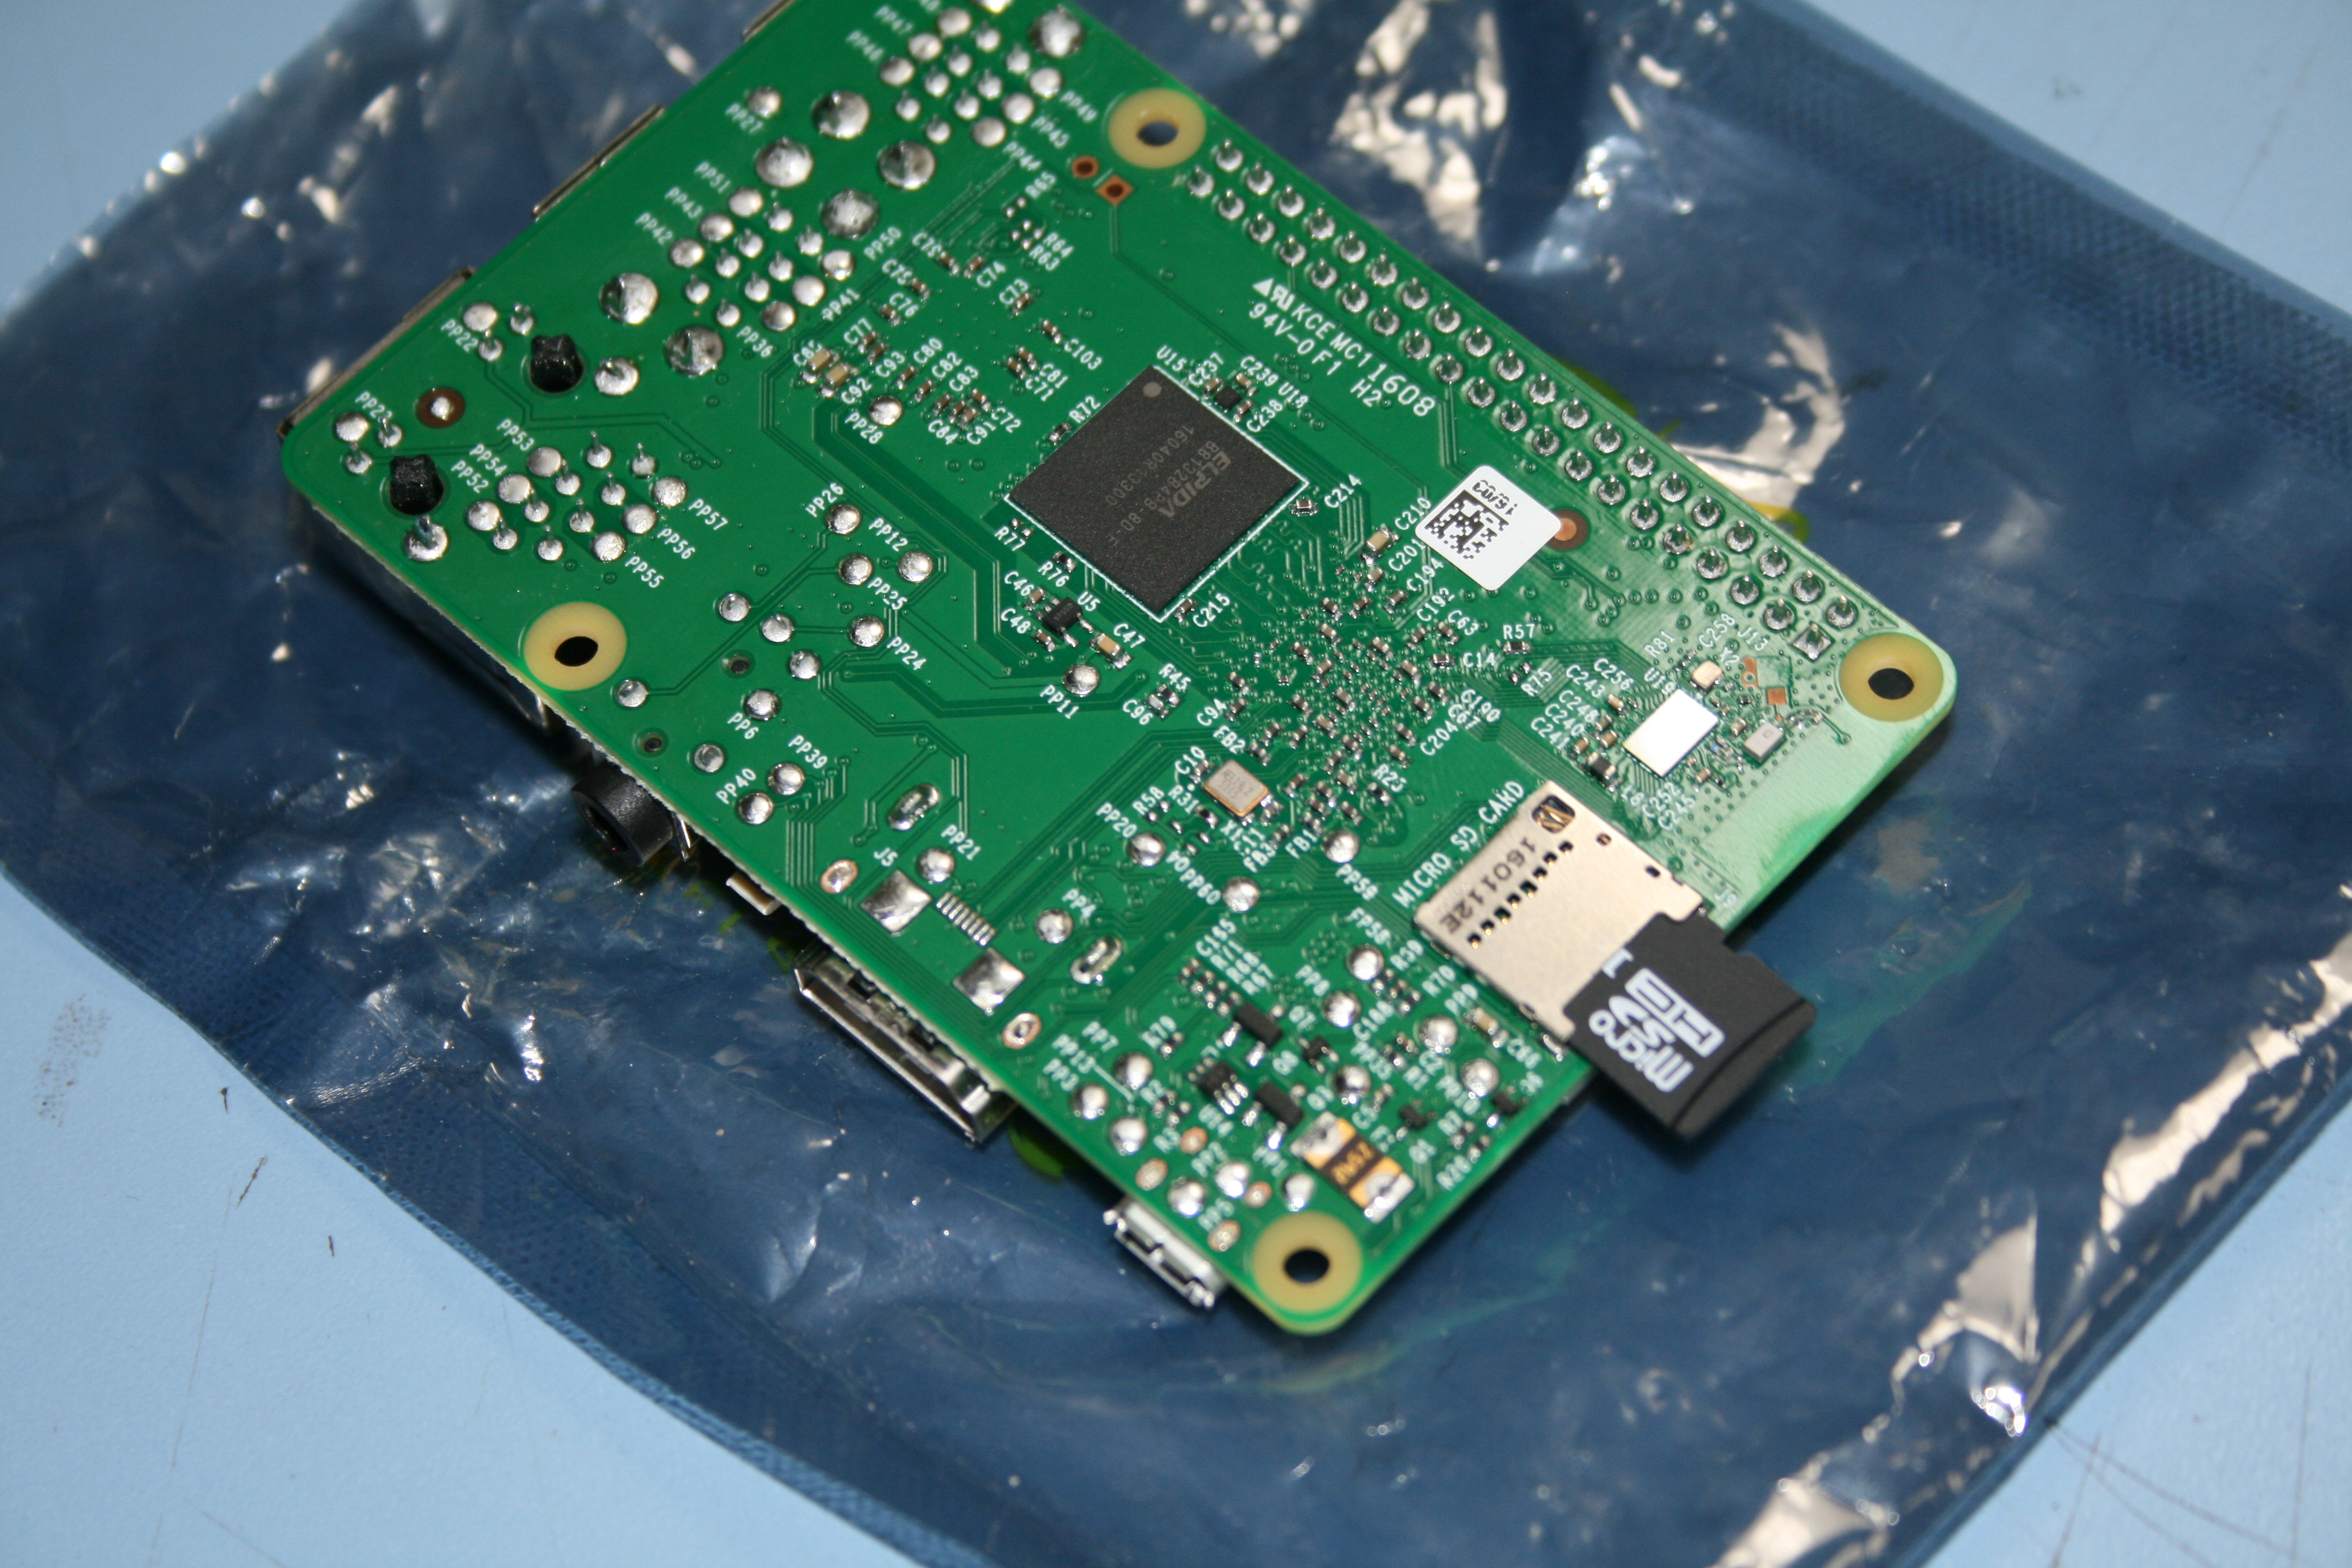
\includegraphics[width=.6\paperwidth]{images/microsd.jpg}}
\end{center}
	\caption{ \textit{La \textit{RaspberryPi} de dos}}
\end{figure}\\

	\item Ensuite, nous allons pouvoir lancer la \textit{RaspberryPi}. Avant de l'alimenter, nous allons distinguer deux cas.. Si vous avez la possibilité, de façon extérieur, d'accéder à l'adresse IP de votre \textit{RaspberryPi} alors vous pouvez sauter l'étape N°3. Si cela n'est pas possible, brancher un écran et un clavier.\\
	Vous pouvez maintenant l'alimenter en utilisant le port micro USB qui est à côté du port HDMI.\\
	
	\item Si vous suivez cette étape, vous devriez voir apparaître des lignes de commandes qui défilent. Quelques instants plus tard, vous arrivez sur l'environnement de bureau de votre \textit{RaspberryPi}.\\
	% faire la demarche pour ouvrir un terminal.
Une fois le terminal ouvert, entrer la commande suivante :\\
\begin{lstlisting}[style=MyBashStyle]
	sudo ifconfig
\end{lstlisting}
un mot de passe devrait vous être demandé, par défaut, le mot de passe est "robots1234"

	\item Très bien, désormais que vous avez l'adresse IP à disposition, nous allons pouvoir installer le nécessaire pour utiliser nos capteurs. Nous aurions très bien pu continuer cette installation directement sur la \textit{RaspberryPi} mais si vous n'avez jamais fait ce qui va suivre, cela vous fera un bon entrainement.\\

\begin{enumerate} 
	\item Télécharger le logiciel \href{https://git-for-windows.github.io/}{Git Bash}
	\item Lancer \textit{Git Bash}
	\item taper la commande en remplaçant "xxx.xxx.xxx.xxx" par l'adresse IP de la \textit{RaspberryPi}\\
	\begin{lstlisting}[style=MyBashStyle]
	ssh pi@xxx.xxx.xxx.xxx
	\end{lstlisting}\\
la première fois, il vous sera demander si vous faites confiante, taper alors "yes" puis sur \textit{Entrée}
	\item Le mot de passe est "robots1234". Si tout c'est bien passé, vous devriez avoir cet aperçu :
	
	\item vous naviguez maintenant dans la \textit{RaspberryPi}. Dans un premier temps, nous allons changer le mot de passe car celui ci est un mot de passe par défaut. Enter la commande :\\
	\begin{lstlisting}[style=MyBashStyle]
	sudo raspi-config
	\end{lstlisting}\\
	un écran bleu devrait apparaître. %insérer image ici et expliquer le chmt mdp et expand
	
	\item Quitter le menu pour revenir au terminal.
	\item Maintenant, nous allons installer GrovePi+ pour pouvoir utiliser le \textit{Shield}. Entrer alors les deux commandes suivantes :\\
	\begin{lstlisting}[style=MyBashStyle]
	sudo curl https://raw.githubusercontent.com/DexterInd
	/Raspbian_For_Robots/master/upd_script/fetch_grovepi.sh | bash
	 
	sudo reboot
	\end{lstlisting}\\
	Votre \textit{RaspberryPi} va redémarrer.
	\item Connecter vous à nouveau en "ssh" comme pour l'étape 4 mais cette fois ci avec votre nouveau mot de passe.
	\item Réaliser alors cette suite de commande une à une. Appuyer sur la touche \textit{Entrée} lorsque l'on vous demande de continuer :
	\begin{lstlisting}[style=MyBashStyle]
	cd /home/pi/Desktop
	sudo git clone https://github.com/DexterInd/GrovePi
	cd /home/pi/Desktop/GrovePi/Script
	sudo chmod +x install.sh
	sudo ./install.sh
	\end{lstlisting}\\
	
	\item Appuyez à nouveau sur \textit{Entrée} une fois arrivé sur cette configuration :
	%insérer image
	\item Au moment où la \textit{RaspberryPi} va redémarrer (vous verrez un "Restart" écrit dans le terminal. Appuyez sur \textit{Ctrl + C} pour empêcher le redémarrage.
	\item Effectuer alors la commande :
	\begin{lstlisting}[style=MyBashStyle]
	sudo shutdown now
	\end{lstlisting}\\
	Elle va alors s'arrêter. Vous pouvez alors la débrancher une fois que vous avez un écran noir.
	\end{enumerate}\\
	
		\item Vous pouvez désormais ajouter le \textit{Shield} sur la \textit{RaspberryPi} Comme ci-dessous \textbf{ATTENTION AU BROCHES UTILISÉES SUR LA PHOTO !}\\
		%inserer photo branchement grovepi
		\item Brancher à nouveau la \textit{RaspberryPi}. Vous devriez avoir une LED qui s'allume sur votre \textit{Shield}
		\item nous allons tester s'il a bien été reconnue, pour cela, connecter vous en "ssh" sur votre \textit{RaspberryPi} (vous devriez savoir le faire maintenant !)
		\item lancer la commande :
		\begin{lstlisting}[style=MyBashStyle]
		sudo i2cdetect -y 1
		\end{lstlisting}\\
	
vous devriez obtenir ce résultat, avec le 04 en première ligne. %ajouter image

\end{enumerate}\\

Voilà, la première mise en route de la \textit{RaspberryPi} est terminé, nous allons maintenant pouvoir nous occuper du code pour la station final.

\section{Installation, configuration et test du code de la station avec ses capteurs.}\\

\subsection{Installation des capteurs.}\\

Votre \textit{RaspberryPi} est configurée, ainsi que son \textit{Shield}. Nous allons maintenant pouvoir installer les différents capteurs. Regardons de plus près les différents connecteurs. %mettre une photo du shield
\\
Comme vous pouvez le voir, il y a écrit un numéro d'identification du connecteur sur le \textit{Shield}. Vous allez donc brancher sur des ports particulier en adéquation avec le code qui sera télécharger ultérieurement.\\

Vous allez faire les branchements suivants :
\begin{enumerate}
	\item Le capteur de température et d'humidité sur le port D7. %mettre une photo
	\item Le capteur de luminosité sur le port A1. %mettre une photo
	\item L'encodeur rotatif sur le port A2. %mettre une photo
	\item L'écran LCD sur un des ports I2C. %mettre une photo
\end{enumerate}\\

Vous devriez alors obtenir un résultat similaire à celui là : %photo

\subsection{Configuration de la \textit{RaspberryPi}.}\\

Nous allons maintenant télécharger le code pour activer le station. Pour cela, brancher votre \textit{RaspberryPi} au secteur et au réseau si jamais vous aviez enlevé le câble ethernet. Connectez vous en \textit{ssh} via \textit{git bash} et exécutez la commande : 
%mettre la commande git clone du repo final

\\
Cette commande va télécharger le code nécessaire au fonctionnement de la station. Nous modifierons ce code dans le troisième chapitre pour envoyer les données sur le \textit{Cloud}.\\
Tapez la commande :

vous devriez voir apparaitre un dossier %nomdudossierdurepo.
Si cela n'est pas le cas, réessayer la commande précédente.
Nous allons maintenant modifier un fichier dans \textit{Raspbian} pour faire en sorte que le script qui gère les capteurs puisse se lancer au démarrage de la \textit{RaspberryPi}.\\

Exécuter la commande : 
%commande rc local /home/pi/repogit/.../machin.py &
\\
Ajouter alors la ligne : 
%ligne
\\

\subsection{Test de la station}\\

Vous allez tout d'abord essayer la station en lançant le script manuellement pour vérifier que cela fonctionne, puis nous redémarrerons la \textit{RaspberryPi} pour voir si la modification de l'étape précédente est fonctionnelle.

Tapez alors la commande suivante pour aller dans le dossier. %commande cd
\\
Puis taper la commande %Sudo python .....py

Vous devriez voir l'écran qui s'allume avec le message "Bienvenue dans l'IoT Hub" pendant quelques seconde puis un des menus qui affiche les données des capteurs. Si cela reste sur le premier message, tourner l'encodeur rotatif pour afficher les menus.

Si vous voyez bien tous les menus avec une valeur, on y est, la station fonctionne. Nous allons maintenant vérifier qu'elle démarre bien en même temps que la \textit{RaspberryPi}.
Mettons nous dans le scénario où elle a été coupé électriquement. 
Taper la commande : %shutdown now.
Patienter quelques instants, débrancher puis rebrancher là. Vous devriez alors voir l'écran s'allumer comme pour le test précédent au bout d'un certain temps. %image.

Et voilà, nous arrivons au terme de ce chapitre, vous avez désormais une station fonctionnelle localement. Je vous invite alors à suivre le chapitre trois pour configurer \textit{Microsoft Azure} d'une part puis pour modifier le code de tel sorte qu'il envoie les messages sur \textit{le Cloud Azure}.



	
	

%\input{./interface.tex}
%\input{./resolution.tex}
%\input{./computervision.tex}
%\input{./conclusion.tex}
\newpage
%récupérer les citation avec "/footnotemark"
\nocite{*}
%choix du style de la biblio
\bibliographystyle{plain}
%inclusion de la biblio
%\bibliography{bibliographie.bib}
%voir wiki pour plus d'information sur la syntaxe des entrées d'une bibliographie
\end{document}